\documentclass[]{article}
\usepackage{lmodern}
\usepackage{amssymb,amsmath}
\usepackage{ifxetex,ifluatex}
\usepackage{fixltx2e} % provides \textsubscript
\ifnum 0\ifxetex 1\fi\ifluatex 1\fi=0 % if pdftex
  \usepackage[T1]{fontenc}
  \usepackage[utf8]{inputenc}
\else % if luatex or xelatex
  \ifxetex
    \usepackage{mathspec}
  \else
    \usepackage{fontspec}
  \fi
  \defaultfontfeatures{Ligatures=TeX,Scale=MatchLowercase}
\fi
% use upquote if available, for straight quotes in verbatim environments
\IfFileExists{upquote.sty}{\usepackage{upquote}}{}
% use microtype if available
\IfFileExists{microtype.sty}{%
\usepackage{microtype}
\UseMicrotypeSet[protrusion]{basicmath} % disable protrusion for tt fonts
}{}
\usepackage[margin=1in]{geometry}
\usepackage{hyperref}
\hypersetup{unicode=true,
            pdftitle={Simulation Fixed Effect},
            pdfauthor={Xuelong Wang},
            pdfborder={0 0 0},
            breaklinks=true}
\urlstyle{same}  % don't use monospace font for urls
\usepackage{graphicx,grffile}
\makeatletter
\def\maxwidth{\ifdim\Gin@nat@width>\linewidth\linewidth\else\Gin@nat@width\fi}
\def\maxheight{\ifdim\Gin@nat@height>\textheight\textheight\else\Gin@nat@height\fi}
\makeatother
% Scale images if necessary, so that they will not overflow the page
% margins by default, and it is still possible to overwrite the defaults
% using explicit options in \includegraphics[width, height, ...]{}
\setkeys{Gin}{width=\maxwidth,height=\maxheight,keepaspectratio}
\IfFileExists{parskip.sty}{%
\usepackage{parskip}
}{% else
\setlength{\parindent}{0pt}
\setlength{\parskip}{6pt plus 2pt minus 1pt}
}
\setlength{\emergencystretch}{3em}  % prevent overfull lines
\providecommand{\tightlist}{%
  \setlength{\itemsep}{0pt}\setlength{\parskip}{0pt}}
\setcounter{secnumdepth}{5}
% Redefines (sub)paragraphs to behave more like sections
\ifx\paragraph\undefined\else
\let\oldparagraph\paragraph
\renewcommand{\paragraph}[1]{\oldparagraph{#1}\mbox{}}
\fi
\ifx\subparagraph\undefined\else
\let\oldsubparagraph\subparagraph
\renewcommand{\subparagraph}[1]{\oldsubparagraph{#1}\mbox{}}
\fi

%%% Use protect on footnotes to avoid problems with footnotes in titles
\let\rmarkdownfootnote\footnote%
\def\footnote{\protect\rmarkdownfootnote}

%%% Change title format to be more compact
\usepackage{titling}

% Create subtitle command for use in maketitle
\newcommand{\subtitle}[1]{
  \posttitle{
    \begin{center}\large#1\end{center}
    }
}

\setlength{\droptitle}{-2em}

  \title{Simulation Fixed Effect}
    \pretitle{\vspace{\droptitle}\centering\huge}
  \posttitle{\par}
    \author{Xuelong Wang}
    \preauthor{\centering\large\emph}
  \postauthor{\par}
      \predate{\centering\large\emph}
  \postdate{\par}
    \date{2018-07-18}

\usepackage{booktabs}
\usepackage{longtable}
\usepackage{array}
\usepackage{multirow}
\usepackage[table]{xcolor}
\usepackage{wrapfig}
\usepackage{float}
\usepackage{colortbl}
\usepackage{pdflscape}
\usepackage{tabu}
\usepackage{threeparttable}
\usepackage{threeparttablex}
\usepackage[normalem]{ulem}
\usepackage{makecell}

\usepackage{float,amsmath, bbm, siunitx, bm}
\floatplacement{figure}{H}
\newcommand{\indep}{\rotatebox[origin=c]{90}{$\models$}}

\begin{document}
\maketitle

{
\setcounter{tocdepth}{2}
\tableofcontents
}
\section{Motivation}\label{motivation}

Based on the previous simulation results, the interaction effect
estimation is biased. One possible reason is that we consider the
\(\beta's\) as random effects, which will affect the covariance
structure of the signals. More specifically, If \(\beta\) is fixed, then
we have following \[
  Var(X\beta) = \beta^T\Sigma_{X}\beta,
\] Where \(\Sigma_{X} = Var(X)\). We can see that the X's covariance has
an affect on the signal's variance.

However, if we consider \(\beta\) as an random effect, then
\(Var(X\beta)\) is not only related with \(X\) but also with \(\beta's\)
covariance. Therefore, in the following simulation the \(\beta\) is
fixed and there is no average out summary across different values of
\(\beta\).

\section{Simulation result}\label{simulation-result}

\subsection{Setup}\label{setup}

In the following simulation, I just randomly generated 3 different sets
of values for \(\beta\) (main and interaction) . Give each set of
\(\beta's\), the values of y is generated 100 times and thus 100
estimations of variance of main effects and interaction effects.

\subsection{Full data}\label{full-data}

\subsubsection{Averaged estimation}\label{averaged-estimation}

\rowcolors{2}{gray!80}{white}

\begin{table}[!h]

\caption{\label{tab:full data}null-full}
\centering
\begin{tabular}[t]{r|r|r|r|r|r}
\hiderowcolors
\hline
true\_main & true\_interaction & GCTA\_main & GCTA\_interaction & prop\_main & prop\_interaction\\
\hline
\showrowcolors
3.2158113 & 49.40766 & 4.3544031 & 9.8020884 & 6.3131046 & 19.9637333\\
\hline
0.0000000 & 0.00000 & 1.7708630 & 0.3238356 & 1.3104548 & 0.5987790\\
\hline
1.4348505 & 13.20353 & 4.2029131 & 0.5565153 & 8.8826209 & 1.8856730\\
\hline
0.0000000 & 0.00000 & 0.7651304 & 0.0759305 & 0.7295852 & 0.2124003\\
\hline
0.8500824 & 29.33039 & 9.0731883 & 3.6950261 & 11.2518946 & 3.9226269\\
\hline
0.0000000 & 0.00000 & 1.3603169 & 0.2463424 & 1.1417417 & 0.2855682\\
\hline
\end{tabular}
\end{table}

\rowcolors{2}{white}{white} \rowcolors{2}{gray!80}{white}

\begin{table}[!h]

\caption{\label{tab:full data}rank-full}
\centering
\begin{tabular}[t]{r|r|r|r|r|r}
\hiderowcolors
\hline
true\_main & true\_interaction & GCTA\_main & GCTA\_interaction & prop\_main & prop\_interaction\\
\hline
\showrowcolors
2.6873762 & 4.291104 & 2.8521057 & 5.6127113 & 2.9875348 & 0.8293864\\
\hline
0.0000000 & 0.000000 & 0.5219216 & 0.9289016 & 0.4989542 & 0.4139479\\
\hline
1.5461695 & 1.903794 & 0.7875891 & 0.8296039 & 1.8003643 & 0.2571868\\
\hline
0.0000000 & 0.000000 & 0.2677982 & 0.2455065 & 0.3886742 & 0.2667834\\
\hline
0.4947499 & 5.449791 & -0.0100967 & 4.7920416 & 1.1578751 & 0.4965576\\
\hline
0.0000000 & 0.000000 & 0.0475158 & 0.6945106 & 0.2787832 & 0.2714290\\
\hline
\end{tabular}
\end{table}

\rowcolors{2}{white}{white} \rowcolors{2}{gray!80}{white}

\begin{table}[!h]

\caption{\label{tab:full data}quantile-full}
\centering
\begin{tabular}[t]{r|r|r|r|r|r}
\hiderowcolors
\hline
true\_main & true\_interaction & GCTA\_main & GCTA\_interaction & prop\_main & prop\_interaction\\
\hline
\showrowcolors
2.808878 & 6.248359 & 4.2725694 & 7.1142656 & 5.1323716 & 2.7324792\\
\hline
0.000000 & 0.000000 & 0.6741903 & 0.8282731 & 0.6488152 & 0.5126386\\
\hline
1.493517 & 2.945494 & 1.3331202 & 0.8386872 & 2.5937373 & 0.6850581\\
\hline
0.000000 & 0.000000 & 0.3637601 & 0.2097083 & 0.4655614 & 0.3297226\\
\hline
0.577709 & 8.209279 & 0.1982071 & 4.9213341 & 2.5304851 & 1.5261274\\
\hline
0.000000 & 0.000000 & 0.2193605 & 0.6382106 & 0.4427720 & 0.3743509\\
\hline
\end{tabular}
\end{table}

\rowcolors{2}{white}{white} \rowcolors{2}{gray!80}{white}

\begin{table}[!h]

\caption{\label{tab:full data}log-full}
\centering
\begin{tabular}[t]{r|r|r|r|r|r}
\hiderowcolors
\hline
true\_main & true\_interaction & GCTA\_main & GCTA\_interaction & prop\_main & prop\_interaction\\
\hline
\showrowcolors
2.6937805 & 6.107954 & 5.0208023 & 7.7236308 & 5.5848707 & 1.3456888\\
\hline
0.0000000 & 0.000000 & 0.7177300 & 0.9656956 & 0.6280478 & 0.3237447\\
\hline
1.6151267 & 2.360681 & 0.5707424 & 0.8223152 & 2.0697999 & 0.3163978\\
\hline
0.0000000 & 0.000000 & 0.2375397 & 0.2171377 & 0.3980136 & 0.2521233\\
\hline
0.5805219 & 6.281979 & 0.0926633 & 3.3529820 & 1.9173150 & 0.4860522\\
\hline
0.0000000 & 0.000000 & 0.1422832 & 0.5058683 & 0.3574811 & 0.2421702\\
\hline
\end{tabular}
\end{table}

\rowcolors{2}{white}{white} \rowcolors{2}{gray!80}{white}

\begin{table}[!h]

\caption{\label{tab:full data}sqrt-full}
\centering
\begin{tabular}[t]{r|r|r|r|r|r}
\hiderowcolors
\hline
true\_main & true\_interaction & GCTA\_main & GCTA\_interaction & prop\_main & prop\_interaction\\
\hline
\showrowcolors
2.8923511 & 16.154550 & 5.8498863 & 11.1069955 & 11.1032750 & 17.2475250\\
\hline
0.0000000 & 0.000000 & 1.0780650 & 0.6580931 & 0.9545424 & 1.0366619\\
\hline
1.3593689 & 4.740357 & 1.6579450 & 0.7002400 & 3.6527756 & 2.2664512\\
\hline
0.0000000 & 0.000000 & 0.4476342 & 0.1572187 & 0.5130434 & 0.5033004\\
\hline
0.6224476 & 11.267165 & 0.5178294 & 3.2208614 & 3.7014124 & 2.2444958\\
\hline
0.0000000 & 0.000000 & 0.4421995 & 0.3660503 & 0.5833727 & 0.2835238\\
\hline
\end{tabular}
\end{table}

\rowcolors{2}{white}{white} \rowcolors{2}{gray!80}{white}

\begin{table}[!h]

\caption{\label{tab:full data}cat-10-full}
\centering
\begin{tabular}[t]{r|r|r|r|r|r}
\hiderowcolors
\hline
true\_main & true\_interaction & GCTA\_main & GCTA\_interaction & prop\_main & prop\_interaction\\
\hline
\showrowcolors
2.6921130 & 4.090163 & 3.2023234 & 5.3127400 & 3.0219314 & 2.3507786\\
\hline
0.0000000 & 0.000000 & 0.5573301 & 0.9149534 & 0.4715617 & 0.6328867\\
\hline
1.4802190 & 2.017695 & 0.7938607 & 1.0346787 & 1.7375762 & 0.9872728\\
\hline
0.0000000 & 0.000000 & 0.2702883 & 0.2869367 & 0.3890169 & 0.4708470\\
\hline
0.5241891 & 5.244097 & -0.0565079 & 4.7258258 & 0.9887204 & 1.3254654\\
\hline
0.0000000 & 0.000000 & 0.0360078 & 0.6983307 & 0.2675379 & 0.4672848\\
\hline
\end{tabular}
\end{table}

\rowcolors{2}{white}{white} \rowcolors{2}{gray!80}{white}

\begin{table}[!h]

\caption{\label{tab:full data}cat-5-full}
\centering
\begin{tabular}[t]{r|r|r|r|r|r}
\hiderowcolors
\hline
true\_main & true\_interaction & GCTA\_main & GCTA\_interaction & prop\_main & prop\_interaction\\
\hline
\showrowcolors
2.7000186 & 3.845413 & 2.9814892 & 4.5664152 & 2.7577871 & 2.3837907\\
\hline
0.0000000 & 0.000000 & 0.5389448 & 0.8707940 & 0.4572031 & 0.6435033\\
\hline
1.5233407 & 2.095205 & 0.6560493 & 1.1843935 & 1.6552562 & 1.4631640\\
\hline
0.0000000 & 0.000000 & 0.2460147 & 0.3280028 & 0.3682952 & 0.5492955\\
\hline
0.5844635 & 5.039599 & -0.0089763 & 4.9405562 & 0.9122658 & 1.7972413\\
\hline
0.0000000 & 0.000000 & 0.0597922 & 0.7460484 & 0.2607959 & 0.5506845\\
\hline
\end{tabular}
\end{table}

\rowcolors{2}{white}{white} \rowcolors{2}{gray!80}{white}

\begin{table}[!h]

\caption{\label{tab:full data}cat-2-full}
\centering
\begin{tabular}[t]{r|r|r|r|r|r}
\hiderowcolors
\hline
true\_main & true\_interaction & GCTA\_main & GCTA\_interaction & prop\_main & prop\_interaction\\
\hline
\showrowcolors
2.7625360 & 4.174994 & 2.7357569 & 4.8980288 & 2.4478650 & 0.4305927\\
\hline
0.0000000 & 0.000000 & 0.5691043 & 1.0556699 & 0.4673456 & 0.2555173\\
\hline
2.0988911 & 2.415461 & 0.6686098 & 1.4511920 & 2.0919194 & 0.2109776\\
\hline
0.0000000 & 0.000000 & 0.2497561 & 0.4816661 & 0.4485330 & 0.1846766\\
\hline
0.8243926 & 4.359497 & 0.0476966 & 7.2911735 & 0.5193437 & 0.6674842\\
\hline
0.0000000 & 0.000000 & 0.0733865 & 1.3249693 & 0.2321657 & 0.2455678\\
\hline
\end{tabular}
\end{table}

\rowcolors{2}{white}{white}

\clearpage

\subsubsection{Histgram of 100
iterations}\label{histgram-of-100-iterations}

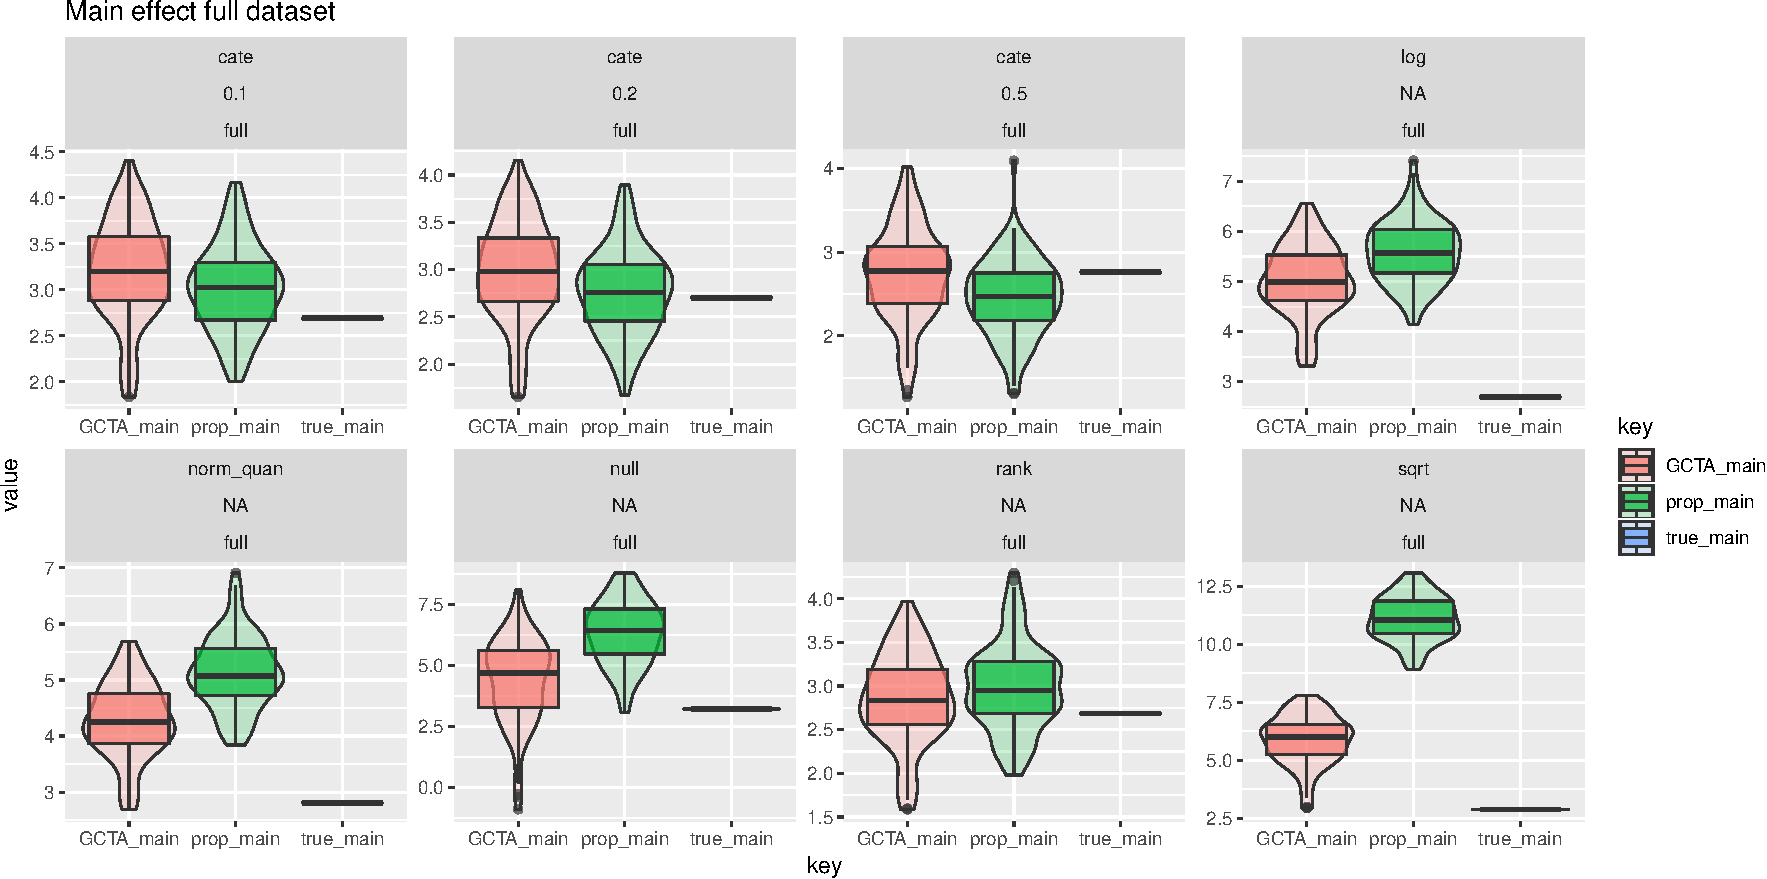
\includegraphics{Fixed_effect_simulation_files/figure-latex/full_main-1.pdf}

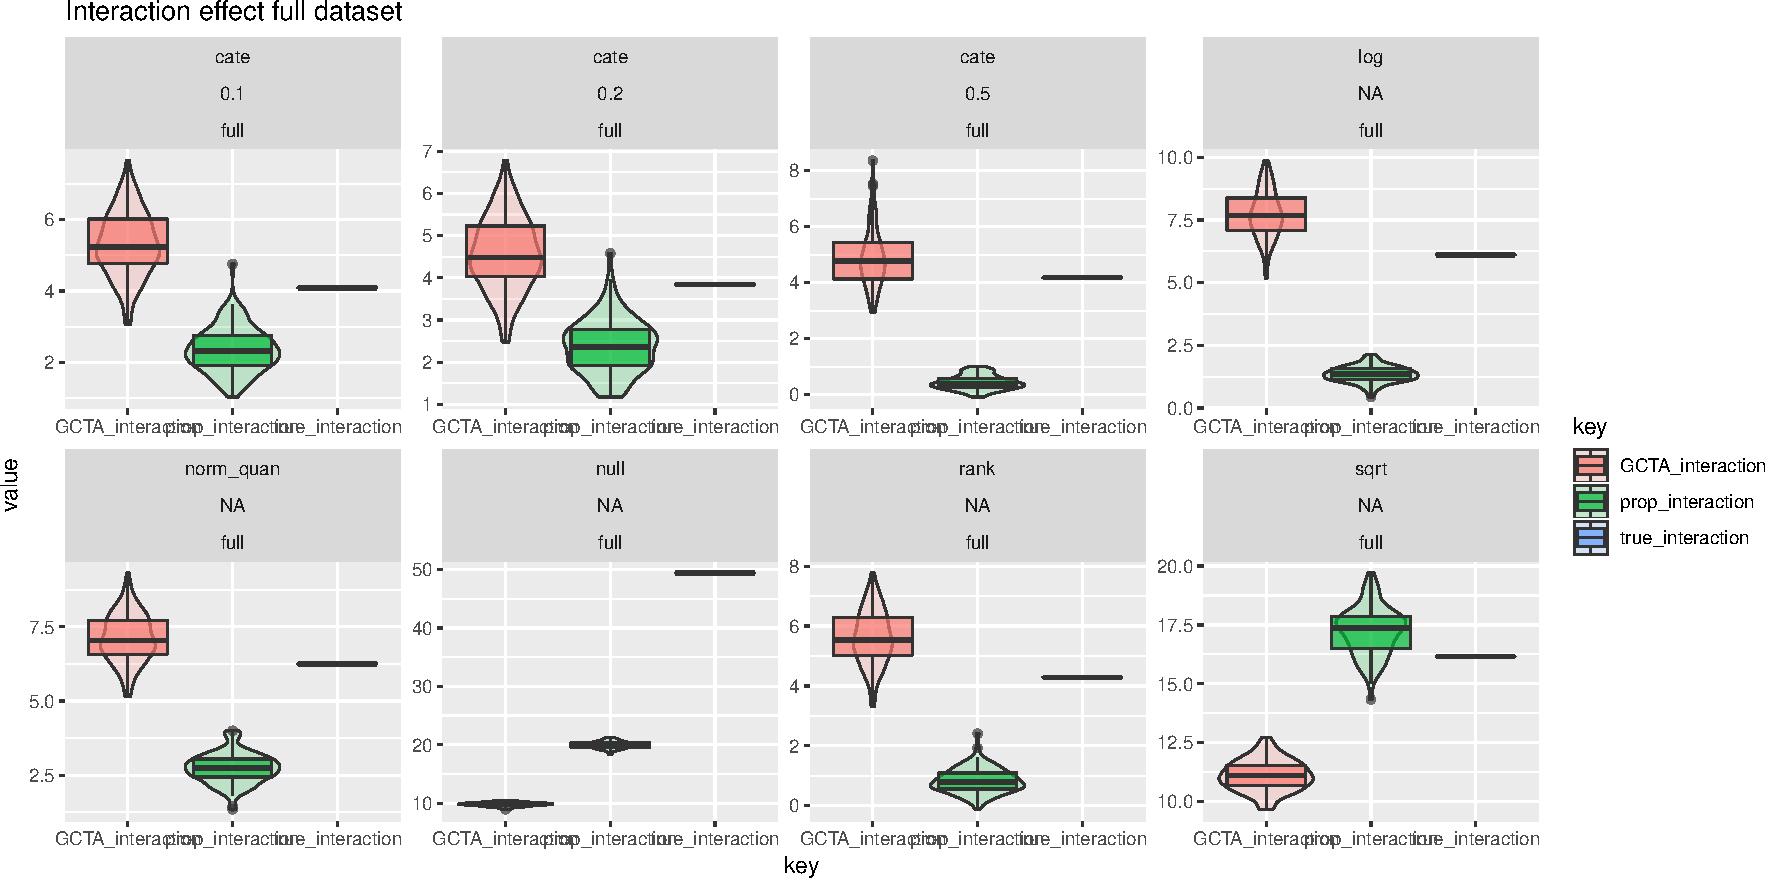
\includegraphics{Fixed_effect_simulation_files/figure-latex/full_inter-1.pdf}

\subsection{Remove 7 subset data}\label{remove-7-subset-data}

\subsubsection{Averaged estimation}\label{averaged-estimation-1}

\rowcolors{2}{gray!80}{white}

\begin{table}[!h]

\caption{\label{tab:sub7 data}null-full}
\centering
\begin{tabular}[t]{r|r|r|r|r|r}
\hiderowcolors
\hline
true\_main & true\_interaction & GCTA\_main & GCTA\_interaction & prop\_main & prop\_interaction\\
\hline
\showrowcolors
2.326047 & 11.04140 & 2.9874170 & 1.1487788 & 8.6919450 & 1.4596337\\
\hline
0.000000 & 0.00000 & 0.8428856 & 0.1439049 & 0.7281087 & 0.1605680\\
\hline
1.201223 & 43.48742 & -0.7370419 & 7.7927874 & 14.1694376 & 5.0495201\\
\hline
0.000000 & 0.00000 & 1.4242304 & 0.3720183 & 1.0371484 & 0.2705839\\
\hline
1.012090 & 10.01595 & 1.2742855 & 1.4205766 & 5.6320471 & 1.8196181\\
\hline
0.000000 & 0.00000 & 0.6075589 & 0.1547535 & 0.7061331 & 0.1748635\\
\hline
\end{tabular}
\end{table}

\rowcolors{2}{white}{white} \rowcolors{2}{gray!80}{white}

\begin{table}[!h]

\caption{\label{tab:sub7 data}rank-full}
\centering
\begin{tabular}[t]{r|r|r|r|r|r}
\hiderowcolors
\hline
true\_main & true\_interaction & GCTA\_main & GCTA\_interaction & prop\_main & prop\_interaction\\
\hline
\showrowcolors
2.3586213 & 1.7099875 & 3.4010825 & 0.5564496 & 2.9142539 & 0.1923090\\
\hline
0.0000000 & 0.0000000 & 0.5509228 & 0.1968368 & 0.4829440 & 0.2634942\\
\hline
0.8726516 & 4.8404613 & 0.4423640 & 6.9471978 & 0.8599029 & 0.2515139\\
\hline
0.0000000 & 0.0000000 & 0.1999645 & 0.9871361 & 0.3064646 & 0.1832223\\
\hline
0.9815092 & 0.6539307 & 0.9953976 & 0.0356594 & 1.1013735 & -0.0422894\\
\hline
0.0000000 & 0.0000000 & 0.2466602 & 0.0546254 & 0.2439542 & 0.1668013\\
\hline
\end{tabular}
\end{table}

\rowcolors{2}{white}{white} \rowcolors{2}{gray!80}{white}

\begin{table}[!h]

\caption{\label{tab:sub7 data}quantile-full}
\centering
\begin{tabular}[t]{r|r|r|r|r|r}
\hiderowcolors
\hline
true\_main & true\_interaction & GCTA\_main & GCTA\_interaction & prop\_main & prop\_interaction\\
\hline
\showrowcolors
2.3824357 & 2.1391474 & 3.8844804 & 0.6773023 & 3.4683656 & 0.2292941\\
\hline
0.0000000 & 0.0000000 & 0.5892784 & 0.2351244 & 0.5273831 & 0.2151068\\
\hline
0.9031948 & 8.2892384 & -0.1832356 & 8.8315811 & 2.2951339 & 1.0422520\\
\hline
0.0000000 & 0.0000000 & 0.1090191 & 0.9395930 & 0.4331523 & 0.3285844\\
\hline
0.9728945 & 0.9235943 & 1.0575944 & 0.0864704 & 1.2314344 & 0.0207744\\
\hline
0.0000000 & 0.0000000 & 0.2574253 & 0.1056672 & 0.2871658 & 0.1485006\\
\hline
\end{tabular}
\end{table}

\rowcolors{2}{white}{white} \rowcolors{2}{gray!80}{white}

\begin{table}[!h]

\caption{\label{tab:sub7 data}log-full}
\centering
\begin{tabular}[t]{r|r|r|r|r|r}
\hiderowcolors
\hline
true\_main & true\_interaction & GCTA\_main & GCTA\_interaction & prop\_main & prop\_interaction\\
\hline
\showrowcolors
2.3753731 & 2.1161346 & 3.4175941 & 0.5725289 & 3.1828043 & -0.0139009\\
\hline
0.0000000 & 0.0000000 & 0.5604288 & 0.1949268 & 0.4740381 & 0.1380879\\
\hline
1.0225968 & 7.1152262 & -0.1619669 & 6.8799631 & 0.6129037 & 0.4824211\\
\hline
0.0000000 & 0.0000000 & 0.0915385 & 0.8938767 & 0.2883702 & 0.2353967\\
\hline
0.9626496 & 0.9838793 & 1.1858619 & 0.0188071 & 1.3573222 & -0.0626020\\
\hline
0.0000000 & 0.0000000 & 0.2710320 & 0.0669914 & 0.2651128 & 0.1017684\\
\hline
\end{tabular}
\end{table}

\rowcolors{2}{white}{white} \rowcolors{2}{gray!80}{white}

\begin{table}[!h]

\caption{\label{tab:sub7 data}sqrt-full}
\centering
\begin{tabular}[t]{r|r|r|r|r|r}
\hiderowcolors
\hline
true\_main & true\_interaction & GCTA\_main & GCTA\_interaction & prop\_main & prop\_interaction\\
\hline
\showrowcolors
2.3533282 & 4.161740 & 3.9640479 & 1.2051462 & 5.1160571 & 1.1605548\\
\hline
0.0000000 & 0.000000 & 0.6546046 & 0.2669356 & 0.5408662 & 0.1912425\\
\hline
1.0021315 & 17.942518 & -1.3056548 & 8.5014977 & 4.9446045 & 3.4550858\\
\hline
0.0000000 & 0.000000 & 0.6491687 & 0.6615934 & 0.5798050 & 0.3046042\\
\hline
0.9796173 & 1.796764 & 1.6992198 & 0.4067622 & 2.3081148 & 0.6194889\\
\hline
0.0000000 & 0.000000 & 0.3404351 & 0.1760265 & 0.3708196 & 0.1935866\\
\hline
\end{tabular}
\end{table}

\rowcolors{2}{white}{white} \rowcolors{2}{gray!80}{white}

\begin{table}[!h]

\caption{\label{tab:sub7 data}cat-10-full}
\centering
\begin{tabular}[t]{r|r|r|r|r|r}
\hiderowcolors
\hline
true\_main & true\_interaction & GCTA\_main & GCTA\_interaction & prop\_main & prop\_interaction\\
\hline
\showrowcolors
2.3457539 & 1.7426962 & 3.3972965 & 0.6514204 & 2.8515749 & 0.7056741\\
\hline
0.0000000 & 0.0000000 & 0.5548752 & 0.2188062 & 0.4614171 & 0.4096501\\
\hline
0.8910848 & 4.5900370 & 0.3960131 & 6.5894462 & 0.8452006 & 0.8720525\\
\hline
0.0000000 & 0.0000000 & 0.1896358 & 0.9805470 & 0.2703615 & 0.3231284\\
\hline
0.9856932 & 0.6969061 & 1.0796944 & 0.0418221 & 1.1523672 & 0.1498357\\
\hline
0.0000000 & 0.0000000 & 0.2573330 & 0.0588064 & 0.2616573 & 0.3030559\\
\hline
\end{tabular}
\end{table}

\rowcolors{2}{white}{white} \rowcolors{2}{gray!80}{white}

\begin{table}[!h]

\caption{\label{tab:sub7 data}cat-5-full}
\centering
\begin{tabular}[t]{r|r|r|r|r|r}
\hiderowcolors
\hline
true\_main & true\_interaction & GCTA\_main & GCTA\_interaction & prop\_main & prop\_interaction\\
\hline
\showrowcolors
2.3430307 & 1.8309328 & 3.2338604 & 0.5909319 & 2.7097974 & 1.1819612\\
\hline
0.0000000 & 0.0000000 & 0.5517777 & 0.2007778 & 0.4455850 & 0.4850347\\
\hline
0.9577299 & 4.1246182 & 0.4700609 & 6.0277129 & 0.7653511 & 1.4748726\\
\hline
0.0000000 & 0.0000000 & 0.2049841 & 0.9805762 & 0.2545628 & 0.4718127\\
\hline
0.9904863 & 0.7478858 & 1.0610726 & 0.0538243 & 1.0722304 & 0.3622345\\
\hline
0.0000000 & 0.0000000 & 0.2581064 & 0.0648982 & 0.2624449 & 0.3666438\\
\hline
\end{tabular}
\end{table}

\rowcolors{2}{white}{white} \rowcolors{2}{gray!80}{white}

\begin{table}[!h]

\caption{\label{tab:sub7 data}cat-2-full}
\centering
\begin{tabular}[t]{r|r|r|r|r|r}
\hiderowcolors
\hline
true\_main & true\_interaction & GCTA\_main & GCTA\_interaction & prop\_main & prop\_interaction\\
\hline
\showrowcolors
2.419468 & 2.271585 & 3.0376944 & 1.2854136 & 2.4576324 & 0.1298660\\
\hline
0.000000 & 0.000000 & 0.5485878 & 0.2819082 & 0.4326550 & 0.1626354\\
\hline
1.154539 & 2.698032 & 0.4646134 & 3.9490138 & 1.1831423 & 0.9354951\\
\hline
0.000000 & 0.000000 & 0.2102208 & 0.9285393 & 0.3262500 & 0.2752220\\
\hline
1.020003 & 1.312834 & 1.0350381 & 0.2530629 & 1.0065813 & 0.2144515\\
\hline
0.000000 & 0.000000 & 0.2848867 & 0.1596577 & 0.2784719 & 0.1572541\\
\hline
\end{tabular}
\end{table}

\rowcolors{2}{white}{white}

\clearpage

\subsubsection{Histgram of 100
iterations}\label{histgram-of-100-iterations-1}

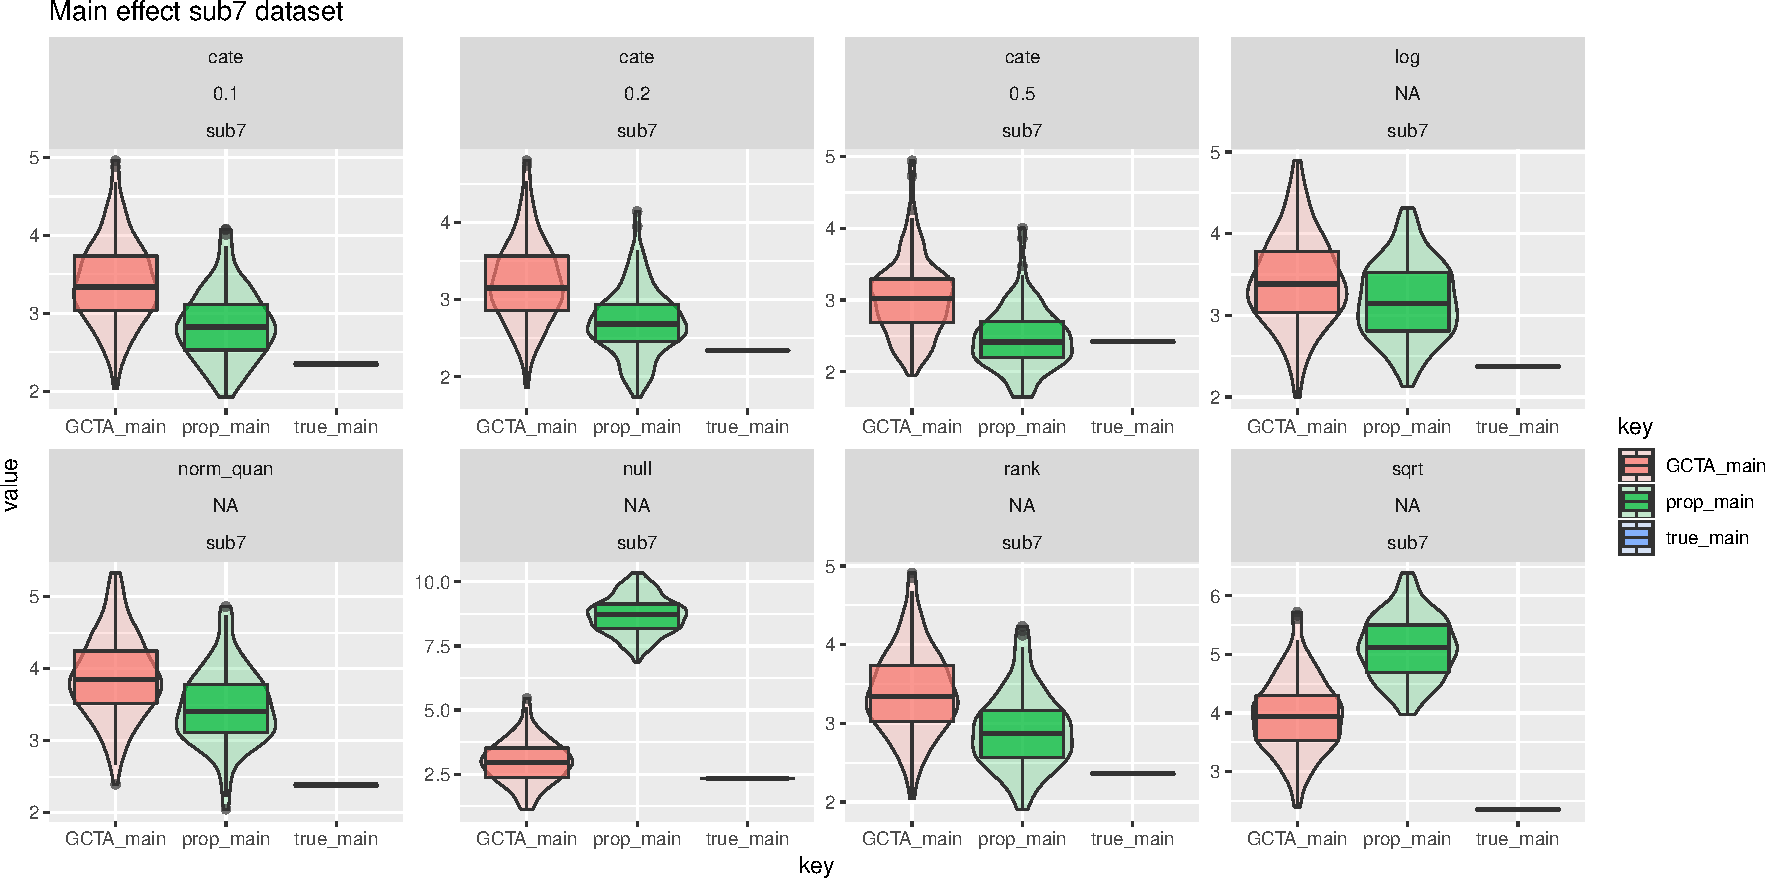
\includegraphics{Fixed_effect_simulation_files/figure-latex/sub7_main-1.pdf}

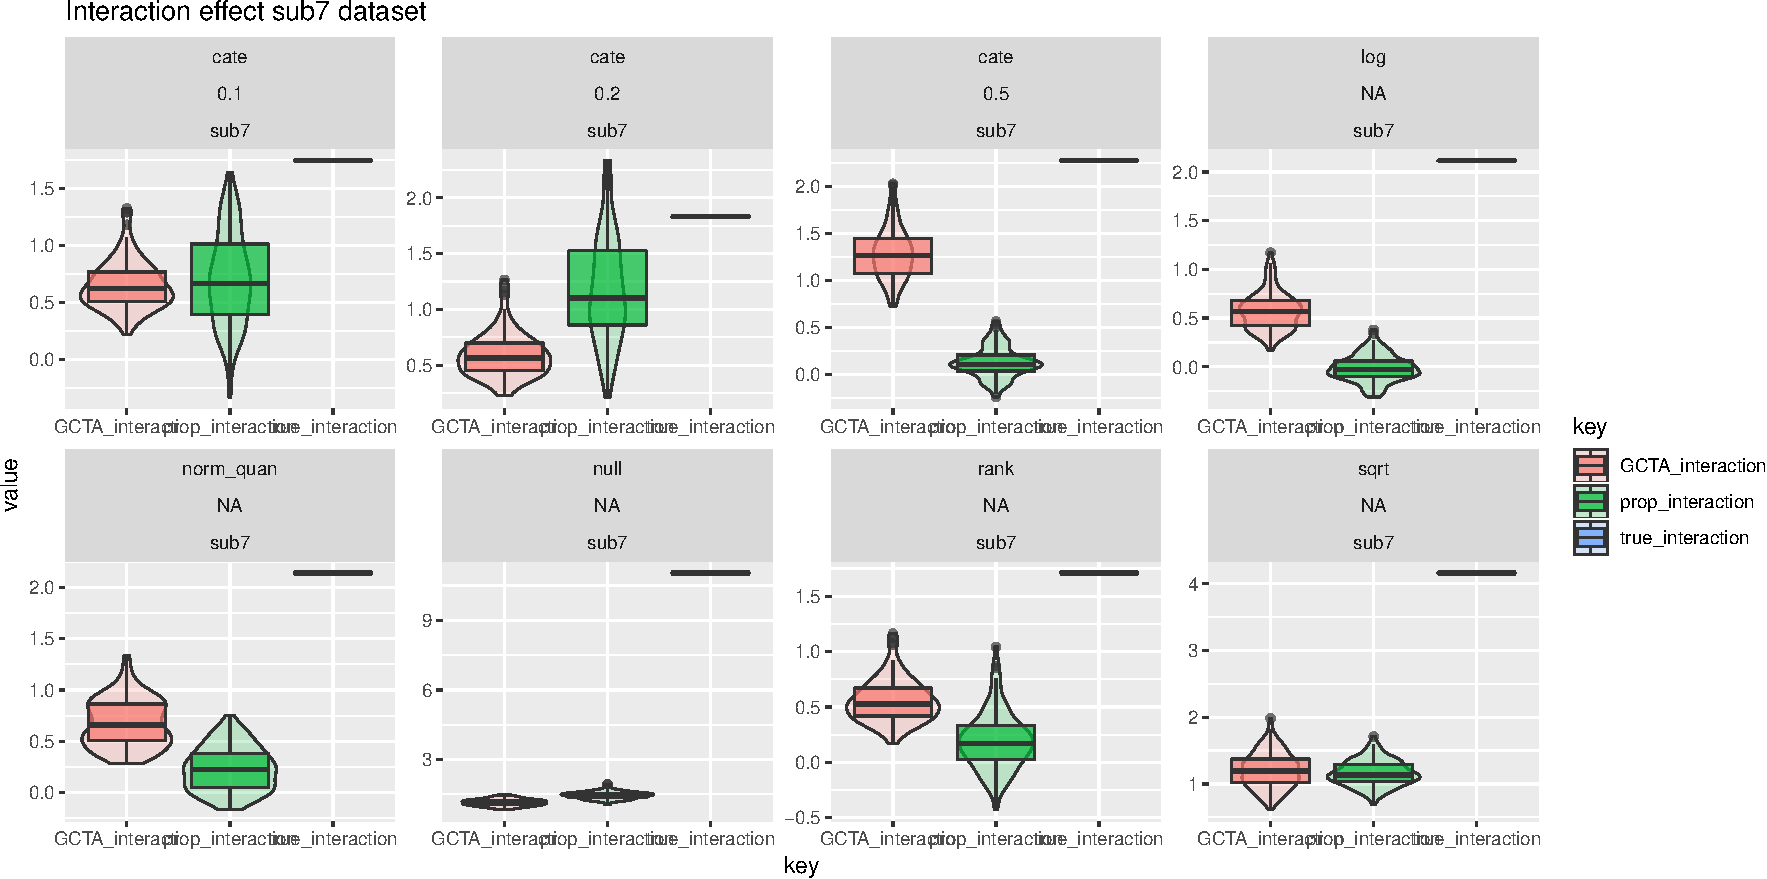
\includegraphics{Fixed_effect_simulation_files/figure-latex/sub7_inter-1.pdf}

\subsection{Remove 11 subset data}\label{remove-11-subset-data}

\subsubsection{Averaged estimation}\label{averaged-estimation-2}

\rowcolors{2}{gray!80}{white}

\begin{table}[!h]

\caption{\label{tab:sub11 data}null-full}
\centering
\begin{tabular}[t]{r|r|r|r|r|r}
\hiderowcolors
\hline
true\_main & true\_interaction & GCTA\_main & GCTA\_interaction & prop\_main & prop\_interaction\\
\hline
\showrowcolors
2.7276371 & 7.708914 & 4.4996190 & 0.4411341 & 5.8478080 & 0.3475610\\
\hline
0.0000000 & 0.000000 & 0.6803805 & 0.0948647 & 0.7255906 & 0.0896674\\
\hline
0.6782210 & 42.661785 & -12.8748992 & 7.1828950 & 6.7056205 & 6.4783280\\
\hline
0.0000000 & 0.000000 & 0.9794912 & 0.3166469 & 1.1283617 & 0.2888135\\
\hline
0.2546506 & 6.389698 & 0.7262481 & 0.3570885 & 1.4882557 & 0.4238215\\
\hline
0.0000000 & 0.000000 & 0.3645878 & 0.0613997 & 0.3866327 & 0.0865650\\
\hline
\end{tabular}
\end{table}

\rowcolors{2}{white}{white} \rowcolors{2}{gray!80}{white}

\begin{table}[!h]

\caption{\label{tab:sub11 data}rank-full}
\centering
\begin{tabular}[t]{r|r|r|r|r|r}
\hiderowcolors
\hline
true\_main & true\_interaction & GCTA\_main & GCTA\_interaction & prop\_main & prop\_interaction\\
\hline
\showrowcolors
2.7824456 & 4.265218 & 3.2448657 & 5.7896516 & 3.3443064 & 0.3522793\\
\hline
0.0000000 & 0.000000 & 0.4651041 & 0.8349188 & 0.4655195 & 0.3027861\\
\hline
0.5280393 & 7.799071 & 0.1915601 & 12.8500545 & 1.0191591 & 0.8875884\\
\hline
0.0000000 & 0.000000 & 0.1012524 & 1.3903298 & 0.3209896 & 0.2369106\\
\hline
0.2060431 & 2.062459 & 0.0258525 & 2.1557215 & 0.3198292 & 0.3661274\\
\hline
0.0000000 & 0.000000 & 0.0471755 & 0.4058309 & 0.2069629 & 0.1993032\\
\hline
\end{tabular}
\end{table}

\rowcolors{2}{white}{white} \rowcolors{2}{gray!80}{white}

\begin{table}[!h]

\caption{\label{tab:sub11 data}quantile-full}
\centering
\begin{tabular}[t]{r|r|r|r|r|r}
\hiderowcolors
\hline
true\_main & true\_interaction & GCTA\_main & GCTA\_interaction & prop\_main & prop\_interaction\\
\hline
\showrowcolors
2.7681842 & 4.328651 & 3.4609212 & 3.1788078 & 3.7258411 & 0.3012130\\
\hline
0.0000000 & 0.000000 & 0.4966609 & 0.4563100 & 0.4782636 & 0.2437290\\
\hline
0.5720811 & 8.861475 & -0.0018297 & 7.9277357 & 1.7294550 & 1.0911548\\
\hline
0.0000000 & 0.000000 & 0.0888270 & 0.7577563 & 0.3681743 & 0.3112944\\
\hline
0.2102370 & 2.610060 & -0.0241759 & 1.7490392 & 0.5688029 & 0.3255822\\
\hline
0.0000000 & 0.000000 & 0.0369378 & 0.3481334 & 0.2419591 & 0.1781135\\
\hline
\end{tabular}
\end{table}

\rowcolors{2}{white}{white} \rowcolors{2}{gray!80}{white}

\begin{table}[!h]

\caption{\label{tab:sub11 data}log-full}
\centering
\begin{tabular}[t]{r|r|r|r|r|r}
\hiderowcolors
\hline
true\_main & true\_interaction & GCTA\_main & GCTA\_interaction & prop\_main & prop\_interaction\\
\hline
\showrowcolors
2.8015527 & 4.236281 & 3.0436241 & 3.1225664 & 2.9212645 & -0.0994888\\
\hline
0.0000000 & 0.000000 & 0.4760496 & 0.4733557 & 0.4227479 & 0.1129165\\
\hline
0.6880008 & 9.662155 & -0.2681637 & 10.3492981 & 1.2794970 & 0.6664158\\
\hline
0.0000000 & 0.000000 & 0.1165141 & 0.9915211 & 0.3792009 & 0.2268278\\
\hline
0.2162960 & 2.792241 & 0.0495233 & 2.1310087 & 0.8529974 & 0.1647751\\
\hline
0.0000000 & 0.000000 & 0.0943554 & 0.4004703 & 0.3055376 & 0.1289602\\
\hline
\end{tabular}
\end{table}

\rowcolors{2}{white}{white} \rowcolors{2}{gray!80}{white}

\begin{table}[!h]

\caption{\label{tab:sub11 data}sqrt-full}
\centering
\begin{tabular}[t]{r|r|r|r|r|r}
\hiderowcolors
\hline
true\_main & true\_interaction & GCTA\_main & GCTA\_interaction & prop\_main & prop\_interaction\\
\hline
\showrowcolors
2.7496796 & 4.991774 & 3.0698755 & 1.5439183 & 3.6669050 & 0.7706162\\
\hline
0.0000000 & 0.000000 & 0.5303200 & 0.2727694 & 0.5097033 & 0.2278629\\
\hline
0.5875359 & 16.125727 & -3.4030933 & 7.2550194 & 3.5858543 & 3.8049015\\
\hline
0.0000000 & 0.000000 & 0.4246016 & 0.5041032 & 0.6744699 & 0.4693367\\
\hline
0.2177059 & 4.100766 & 0.1425676 & 1.0639445 & 1.0052705 & 0.4198141\\
\hline
0.0000000 & 0.000000 & 0.2658448 & 0.1919450 & 0.2954893 & 0.1160203\\
\hline
\end{tabular}
\end{table}

\rowcolors{2}{white}{white} \rowcolors{2}{gray!80}{white}

\begin{table}[!h]

\caption{\label{tab:sub11 data}cat-10-full}
\centering
\begin{tabular}[t]{r|r|r|r|r|r}
\hiderowcolors
\hline
true\_main & true\_interaction & GCTA\_main & GCTA\_interaction & prop\_main & prop\_interaction\\
\hline
\showrowcolors
2.7746561 & 4.240363 & 3.2331377 & 6.0088024 & 3.1935942 & 1.3455091\\
\hline
0.0000000 & 0.000000 & 0.4643888 & 0.8805231 & 0.4701595 & 0.4992688\\
\hline
0.5420920 & 7.563943 & 0.2166931 & 13.1758133 & 0.8792574 & 2.4572655\\
\hline
0.0000000 & 0.000000 & 0.1080425 & 1.4595610 & 0.3151668 & 0.4405500\\
\hline
0.2080076 & 2.064543 & 0.0303424 & 2.2531848 & 0.2375642 & 0.9637317\\
\hline
0.0000000 & 0.000000 & 0.0489175 & 0.4187737 & 0.1802348 & 0.3818249\\
\hline
\end{tabular}
\end{table}

\rowcolors{2}{white}{white} \rowcolors{2}{gray!80}{white}

\begin{table}[!h]

\caption{\label{tab:sub11 data}cat-5-full}
\centering
\begin{tabular}[t]{r|r|r|r|r|r}
\hiderowcolors
\hline
true\_main & true\_interaction & GCTA\_main & GCTA\_interaction & prop\_main & prop\_interaction\\
\hline
\showrowcolors
2.7983825 & 4.074101 & 3.1560364 & 6.1755836 & 2.8901981 & 1.8244826\\
\hline
0.0000000 & 0.000000 & 0.4657834 & 0.9608235 & 0.4291065 & 0.5208825\\
\hline
0.5726266 & 7.321955 & 0.2078162 & 14.0873765 & 0.6228696 & 3.5184265\\
\hline
0.0000000 & 0.000000 & 0.1087906 & 1.6044594 & 0.2741144 & 0.5669474\\
\hline
0.2206165 & 2.011403 & 0.0396105 & 2.3074825 & 0.2352814 & 1.3355904\\
\hline
0.0000000 & 0.000000 & 0.0539100 & 0.4253049 & 0.1751183 & 0.4619231\\
\hline
\end{tabular}
\end{table}

\rowcolors{2}{white}{white} \rowcolors{2}{gray!80}{white}

\begin{table}[!h]

\caption{\label{tab:sub11 data}cat-2-full}
\centering
\begin{tabular}[t]{r|r|r|r|r|r}
\hiderowcolors
\hline
true\_main & true\_interaction & GCTA\_main & GCTA\_interaction & prop\_main & prop\_interaction\\
\hline
\showrowcolors
2.8738907 & 4.081361 & 3.6856333 & 10.4923095 & 3.0103562 & 0.2178511\\
\hline
0.0000000 & 0.000000 & 0.5611821 & 1.7717503 & 0.4416661 & 0.1725719\\
\hline
0.7660228 & 6.637190 & 0.2339092 & 19.1607206 & 0.7280669 & 0.7893286\\
\hline
0.0000000 & 0.000000 & 0.1074537 & 2.4910043 & 0.2514666 & 0.1600060\\
\hline
0.2473301 & 1.650984 & 0.0654467 & 2.1605270 & 0.1597307 & 0.6293876\\
\hline
0.0000000 & 0.000000 & 0.0702851 & 0.6144138 & 0.1620340 & 0.2556775\\
\hline
\end{tabular}
\end{table}

\rowcolors{2}{white}{white}

\clearpage

\subsubsection{Histgram of 100
iterations}\label{histgram-of-100-iterations-2}

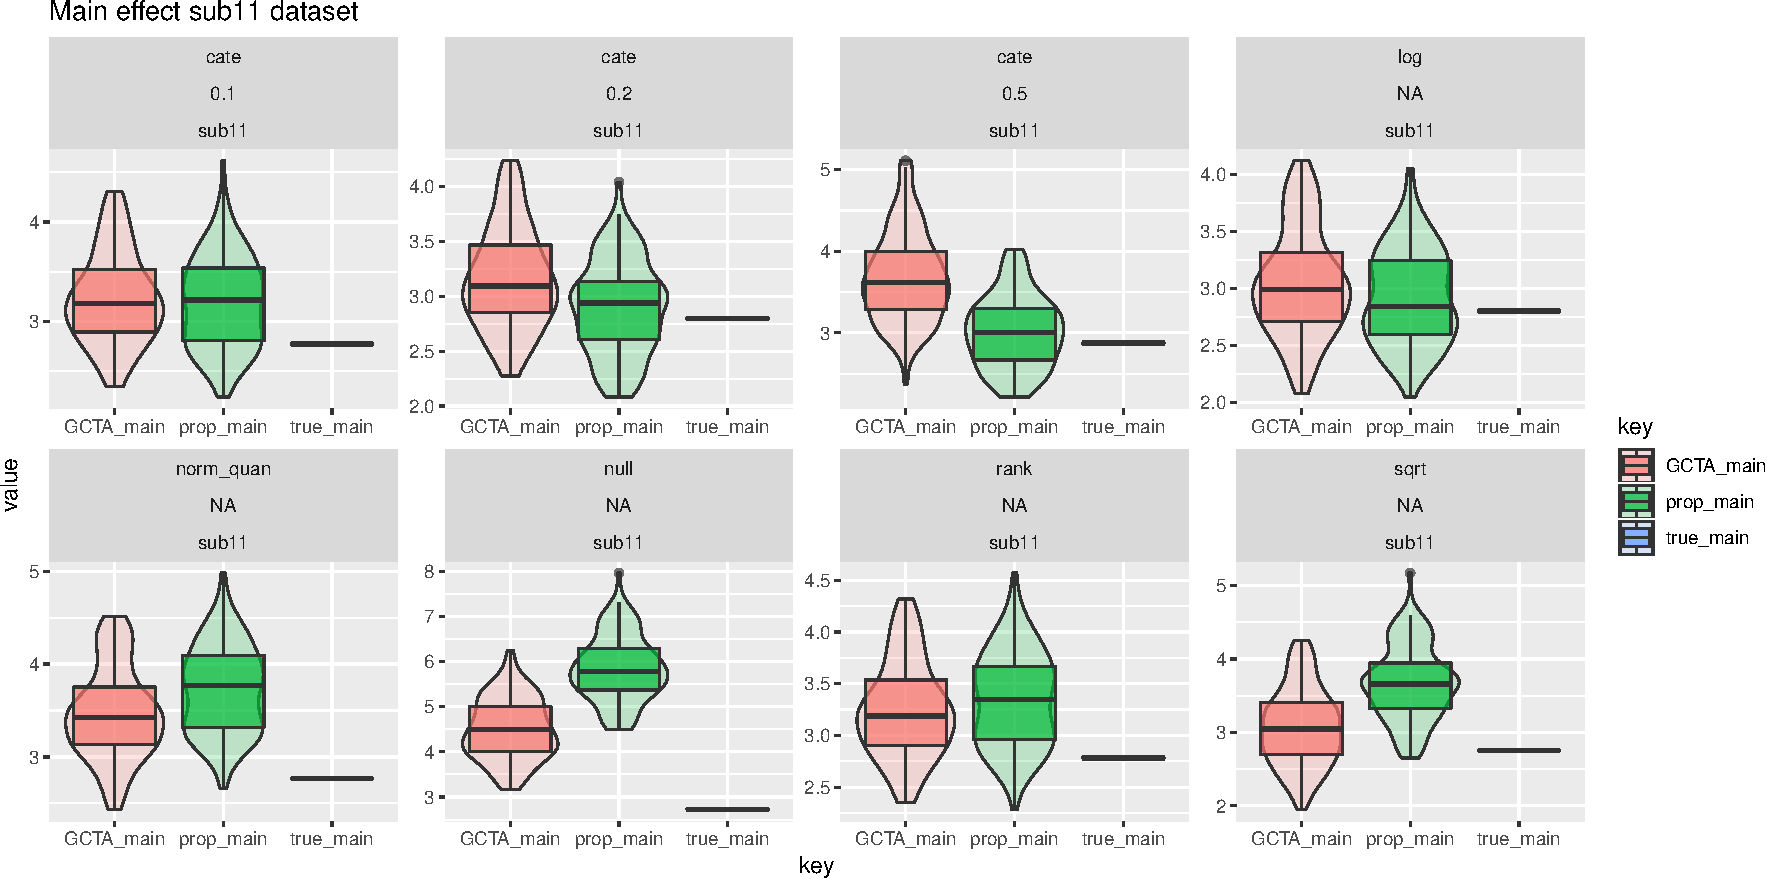
\includegraphics{Fixed_effect_simulation_files/figure-latex/sub11_main-1.pdf}

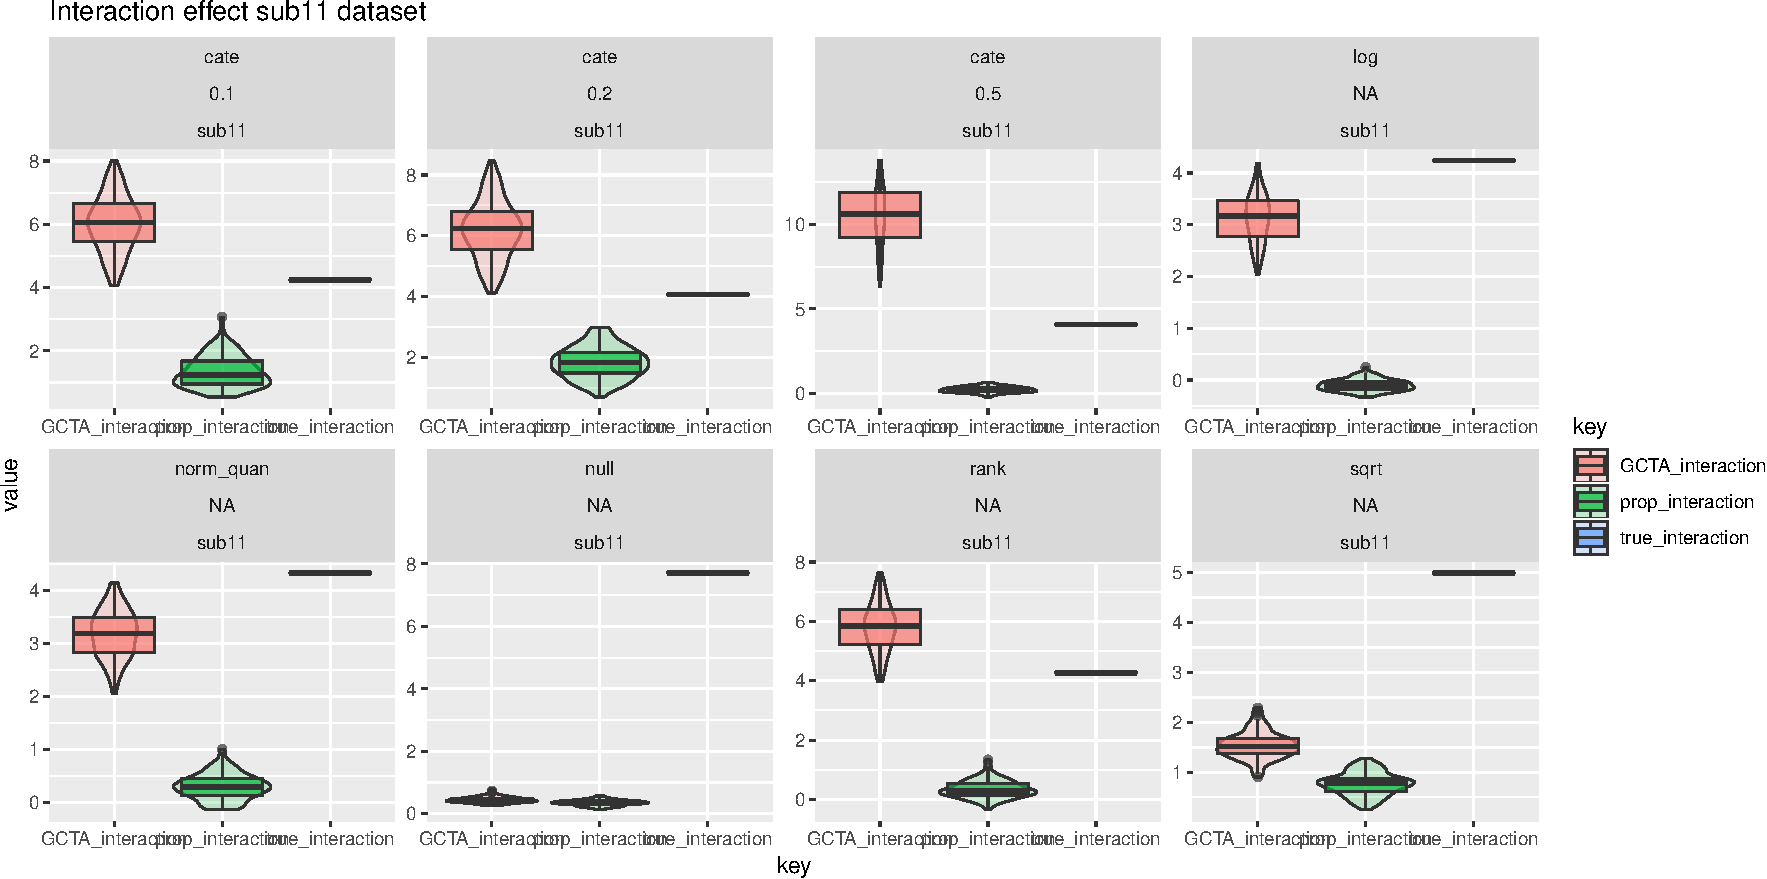
\includegraphics{Fixed_effect_simulation_files/figure-latex/sub11_inter-1.pdf}

\section{Conclusion}\label{conclusion}

\section{Further work}\label{further-work}


\end{document}
